\documentclass[../main.tex]{subfiles}

\begin{document}

\begingroup
\color{midnightblue}
\'E possibile che parte dell'energia interna di una stella alimenti un comportamento oscillatorio attorno alla configurazione di equilibrio. Nei capitoli successivi descrivo la configurazione di equilibrio del Sole e le incertezze nella descrizione fisica del modelo solare standard (MSS).

\endgroup


\begin{figure}[!hb]
    \centering
    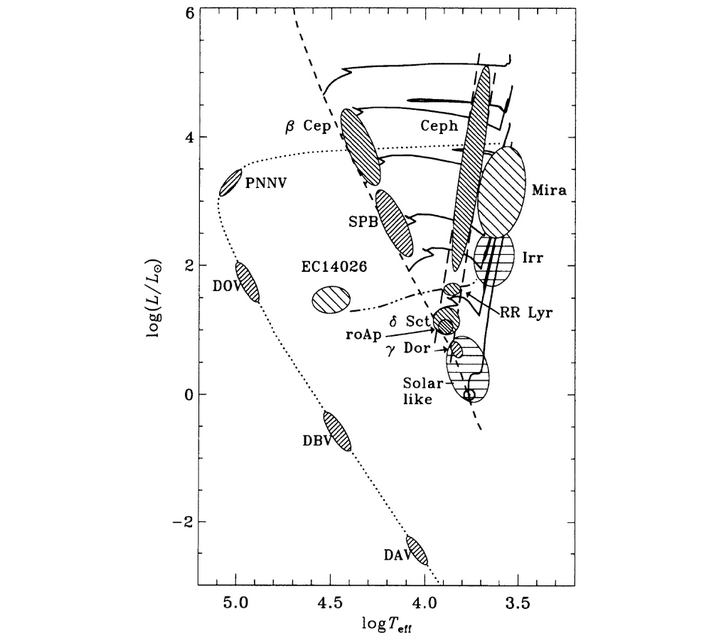
\includegraphics[width=0.5\linewidth]{HRpulsating}
    \caption{Zone del diagramma di \hr{} in cui sono previsti comportamenti oscillatori. Da \cite{chr97lecture}}
    \label{fig:HRp}
\end{figure}


\clearpage


{\let\clearpage\relax \chapter{Strutture autogravitanti in equilibrio}}


\section{Condizione di equilibrio idrostatico.}

\begingroup
\color{midnightblue}
Suppongo che la pressione del campo magnetico, della turbolenza e della radiazione sia molto minore della pressione del gas nell'interno solare e che la correzione dovuta alla rotazione sia piccola; ci\'o \'e suffragato dalla piccola deviazione dalla forma sferica.
\endgroup

La distribuzione di massa del Sole \'e determinata dall'equilibrio tra la forza di attrazione gravitazionale e il gradiente della pressione del gas. Considero una distribuzione di massa sferica con densit\'a $\rho(r,t)$, la variazione della massa presente entro il raggio $r$ \'e descritta da:

\begin{equation}
dm=4\pi r^2\rho \,dr-4\pi r^2\rho v\,dt\label{eq:massvar}
\end{equation}

e $v(r,t)$ \'e il campo di velocit\'a della distribuzione di massa a distanza r dal centro e tempo $t$.

\begingroup
\color{midnightblue}
Eulerian vs Lagrangian description
\endgroup

Per una configurazione di equilibrio statico la velocit\'a radiale del guscio sferico \'e $v=0$ quindi:

\begin{equation}
dm=4\pi r^2\rho \,dr\label{eq:massaguscio}
\end{equation}

Differenziando \eqref{eq:massvar} rispetto alle variabili indipendenti $r$ e $t$ ricavo l'equazione di continuit\'a in coordinate sferiche 
\begin{equation}
\PDy{t}{\rho}=-\frac{1}{r^2}\PDof{r}(\rho r^2 v)
\end{equation}
Per un elemento di fluido qualsiasi, si ha
\begin{equation}
\PDy{t}{\rho}+\nabla\cdot(\rho\vec{v})=0\label{eq:continuityeq}
\end{equation}

Per un gas di particelle debolmente interagenti considero la condizione di equilibrio idrostatico $\ddvec{r}=0$ nella situazione in cui il moto termico delle particelle \'e l'unico contributo al flusso di momento e la forza agente per unit\'a di massa $\vec{f}$ ha solo componente radiale: la conservazione della quantit\'a di moto richiede
\begin{equation}
\rho\TDy{t}{\vec{v}}=-\nabla P+\rho\vec{f}
\end{equation}
da cui ottengo la condizione di equilibrio
\begin{equation}
\nabla P=\rho \vec{f}\label{eq:idrosta}
\end{equation}

Nel caso di una stella la forma della forza per unit\'a di massa f \'e determinata dall'attrazione gravitazionale:

\begin{equation}
g=\frac{Gm(r)}{r^2}\label{eq:gravitya}
\end{equation}
diretta verso il centro di massa.


Definendo il potenziale gravitazionale $\Phi$, soluzione dell'equazione di Poisson 
\begin{equation}
\nabla^2\Phi=4\pi G\rho\label{eq:poisson}
\end{equation}
risulta:
\begin{equation}
\vec{g}=-\PDy{r}{\Phi}=-\frac{Gm(r)}{r^2}\hat{r}
\end{equation}

La condizione di equilibrio idrostatico diventa:
\begin{equation}
\TDy{r}{P}=-\frac{Gm(r)\rho(r)}{r^2}\label{eq:fidroequilibrio}
\end{equation}


\subsection{Tempo di evoluzione dinamico.}

Scrivo l'equazione del moto per la massa $dm$ racchiusa da un guscio sferico di raggio r:
\begin{align}
&\frac{dm}{4\pi r^2}\PtwoDy{t}{r}=f_P+f_g\shortintertext{dove il primo termine sulla destra \'e il contributo dovuto alla differenza di pressione fra i due bordi del guscio, mentre il secondo \'e il contributo della forza di gravit\'a. Esplicitando gli addendi sulla destra e differenziando rispetto a $m$ si ha:}\nonumber\\
&\frac{1}{4\pi r^2}\PtwoDy{t}{r}=-\PDy{m}{P}-\frac{Gm}{4\pi r^4}\label{eq:motionshell}
\end{align}

Per giustificare l'ipotesi di equilibrio idrostatico stimo i tempi caratteristici di evoluzione della struttura solare nel caso la forza dovuta alla pressione o la forza di gravit\'a non fossero bilanciate, approssimando il valore caratteristico della derivata di due variabili con il rapporto del loro valore caratteristico:
\begin{align}
&\tau_{ff}\approx\sqrt{\frac{\rsun{}}{g}}\shortintertext{tempo caratteristico di una distribuzione sferica di materia in caduta libera cio\'e considerando solo il secondo termine in \eqref{eq:motionshell},}\nonumber\\
&\tau_{esp}\approx \rsun{}\sqrt{\frac{\rho}{P}}\shortintertext{tempo caratteristico di espansione dovuta al termine di pressione esclusivamente.}\nonumber
\end{align}

Per i valori
\begin{align}
&G\msun=\num{132712440018+-8}\SI{e9}{\cubic\meter\per\square\second}\\
&\rsun{}=\SI{6.9626+-0.0007}{\meter}
\end{align}
ottengo valori di circa $27$ min.: quindi la costanza delle caratteristiche solari su tempi molto maggiori giustifica l'ipotesi di equilibrio idrostatico, quindi  riscrivo il tempo scala di evoluzione dinamica come

\begin{equation}
\tau_{idro}^{\odot}= \sqrt{\frac{R^3}{GM}}\approx\frac{1}{2}(G\overline{\rho})\expy{-\frac{1}{2}}\approx\SI{27}{\minute}
\end{equation}


\section{Conservazione dell'energia.}

\begingroup
\color{midnightblue}
IL collasso di una nube di gas interstellare \'e un processo complesso; una volta raggiunta una configurazione abbastanza densa, tale che il cammino libero medio degli atomi e dei fotoni sia breve posso considerare il sistema in equilibrio idrostatico e termico. Il processo di collasso gravitazionale continua fino a che l'energia prodotta dalle reazioni nucleari bilancia l'energia irradiata.
\endgroup


\subsection{Teorema del viriale.}

Il teorema del viriale esprime una propriet\'a statistica di particelle interagenti: si trova una relazione tra energia interna, dovuta al moto traslazionale degli atomi, ed energia potenziale gravitazionale, sottointendendo una residua interazione tra le particelle in modo da poter considerare il sistema localmente in equilibrio termodinamico.

\begingroup
\color{grey}
Stimo dall'energia potenziale gravitazionale il valore caratteristico per la velocit\'a del suono all'interno del Sole di circa \SI{400}{\kilo\meter\per\second}.
\endgroup

L'energia potenziale gravitazionale della stella \'e
\begin{equation}
\Omega=-\int_0^M\frac{Gm(r)}{r}\,dm\label{eq:energiapg}
\end{equation}

Il gas solare \'e approssimabile come un gas perfetto monoatomico essendo composto in gran parte da \chem{H} e \chem{^4He} completamente ionizzati quindi l'energia interna \'e costituita dalla somma delle energie traslazionali delle particelle pesate secondo la distribuzione di equilibrio di Maxwell-Boltzmann

\begin{align}
&\int_M\frac{1}{\rho}\int n(\vec{p})\frac{p^2}{2m}\,d\vec{p}\,dm=\frac{3}{2}\int_M\frac{P}{\rho}\,dm\\
&E_i=\int_0^Mu\,dm
\end{align}

dove $n(\vec{p})$ \'e il numero di particelle per unit\'a di volume con impulso in $[\vec{p},\vec{p}+d\vec{p}]$ e u \'e l'energia interna per unit\'a di massa.

Il teorema del viriale 
\begin{equation}
\frac{1}{2}\TtwoDy{t}{I}=2K+\Omega
\end{equation}
con K energia cinetica e $I=\int r^2\,dm$, implica, dato che all'equilibrio $\frac{1}{2}\TtwoDy{t}{I}=0$:

\begin{equation}
0=\int_M\frac{3P}{\rho}\,dm(r)+\Omega
\end{equation}

\begingroup
\color{midnightblue}

Detta $W=E_i+\Omega$ l'energia totale della stella, 
\begin{equation}
\Omega=-2E_i\label{eq:virialegpm}
\end{equation}

e dalla conservazione dell'energia $\TDy{t}{W}+L=0$ segue che durante la fase di collasso prima dell'inizio della sequenza principale met\'a dell'energia gravitazionale viene spesa per aumentare l'energia interna e met\'a in luminosit\'a:

\begin{equation}
L=-\frac{1}{2}\dot{\Omega}=\dot{E}_i
\end{equation}


Il tempo caratteristico che regola il collasso gravitazionale di una massa gassosa in equilibrio idrostatico \'e il tempo di Kelvin-Helmholtz
\begin{equation}
\tkh{}=\frac{\Omega}{L}\approx\frac{GM^2}{2RL}
\end{equation}
sostituendo i valori solari con $\lsun{}=\SI{3.846e33}{\erg\per\second}$ si ha $\tkh{}\approx\SI{1.6e7}{\year}$.

\endgroup

\subsection{Conservazione dell'energia interna}

La prima legge della termodinamica esprime la conservazione dell'energia interna, ovvero mette in relazione il flusso di calore $dq$ per unit\'a di massa in un elemento di gas nell'intervallo di tempo $dt$ con la variazione di energia interna per unit\'a di massa $du$ e di volume specifico $dV$:
\begin{equation}
\TDy{t}{q}=\TDy{t}{u}+P\TDof{t}(\frac{1}{\rho})=0=\TDy{t}{u}+P\TDy{t}{V}\label{eq:prima}
\end{equation}

che posso riscrivere come

\begin{align}
&\TDy{t}{\ln{T}}=\frac{\Gamma_2-1}{\Gamma_2}\TDy{t}{\ln{P}}+\frac{\TDy{t}{q}}{c_PT}\label{eq:primatemp}\\
&\TDy{t}{\ln{P}}=\Gamma_1\TDy{t}{\ln{\rho}}+\frac{\rho(\Gamma_3-1)}{P}\TDy{t}{q}\label{eq:primapres}
\end{align}

dove ho introdotto gli esponenti adiabatici $\Gamma_i$

\begin{equation}
\Gamma_1=\Dcvar{\TDly{\rho}{P}}{Ad}, \ \Gamma_3-1=\Dcvar{\TDly{\rho}{T}}{Ad},\ \frac{\Gamma_2-1}{\Gamma_2}=\Dcvar{\TDly{P}{T}}{Ad}
\end{equation}

\begingroup
\color{midnightblue}

e

tenendo conto del contributo cinetico e dell'energia di ionizzazione di $\cel{H}{1}{}{}$ e $\cel{He}{4}{}{}$ l'energia interna per unit\'a di massa si scrive 

\begin{equation}
u(T,P)=\frac{3\gasconstant{}T}{2\mu}+\frac{1}{\rho}[n_{H^+}\chi_H+n_{He^+}\chi_{He}+n_{He^{++}}(\chi_{He}+\chi_{He^+})]
\end{equation}

con $\chi_x$ energia di ionizzazione dell'atomo $x$ e $n(x^i)$ densit\'a dell'atomo $x$ ionizzato i volte calcolato tramite l'equazione di Saha.

\endgroup


Quando il contributo delle reazioni di fusione o di ionizzazione parziale non \'e trascurabile aggiungo al lato di destra di \eqref{eq:prima} il termine contenente il potenziale chimico $-\mu_idN_i$ con $\mu_i=\Dcvar{\PDy{N_i}{u}}{S,V}$: 

\begingroup
\color{grey}
Il tempo caratteristico che regola il collasso gravitazionale di una massa gassosa in equilibrio idrostatico \'e il tempo di Kelvin-Helmholtz
\begin{equation}
\tkh{}=\frac{\Omega}{L}\approx\frac{GM^2}{2RL}
\end{equation}
sostituendo i valori solari con $\lsun{}=\SI{3.846e33}{\erg\per\second}$ si ha $\tkh{}\approx\SI{1.6e7}{\year}$.
\endgroup

Scrivo il bilancio di calore per un elemento di massa unitaria di gas:

\begin{equation}
\TDy{t}{q}=\epsilon-\frac{1}{\rho}\nabla\cdot\vec{F}\label{eq:heatgl}
\end{equation}
dove $\epsilon$ \'e l'energia prodotta per unit\'a di tempo e massa dalle reazioni nucleari e $\vec{F}$ \'e il flusso di energia verso l'esterno che in situazioni di stabilit\'a dinamica \'e dovuto alla diffusione di fotoni dalla zona pi\'u calda verso la superficie; sostituendo in \eqref{eq:prima} si ha

\begin{equation}
\TDy{r}{L}=4\pi r^2[\rho(\epsilon-\epsilon_{\nu})-\rho\TDof{t}u+\frac{P}{\rho}\TDy{t}{\rho}]\label{eq:fenergyconservation}
\end{equation}

Tengo conto dell'energia generata sotto forma di neutrini, che, alle densit\'a tipiche dell'interno solare, hanno interazioni trascurabili con la materia e quindi non danno luogo a un flusso di calore nel sistema, aggiungendo un termine negativo $\epsilon_{\nu}$ tale che $L_{\nu}=\int_0^M\epsilon_{\nu}\,dm$.

Nel caso stazionario

\begin{equation}
\TDy{t}{q}=0\ \Rightarrow\ dL=4\pi r^2\rho\epsilon\,dr
\end{equation}
e i processi nucleari che avvengono nella parte centrale forniscono il calore per bilanciare il flusso di energia uscente, in particolare le reazioni delle catene $\Pproton\Pproton$ contribuiscono per il $99.9\%$ all'energia generata da reazioni nucleari nel Sole.

Stimo il tempo trascorso da una stella di massa solare in sequenza principale considerando il tempo necessario per la massa di idrogeno nel core di fusione (le temperature necessarie perch\'e il rate di reazione sia apprezzabile si raggiungono nella regione pi\'u interna che costituisce una frazione $f$ pari al $15\%$ della massa solare) a trasformarsi in elio:

\begin{equation}
\tau_n\approx\frac{E_n}{L}=\frac{fX\msun Q}{\lsun}\approx\SI{e+10}{\year}
\end{equation} 
con $Q=\SI{6.3e18}{\erg\per\gram}$.


{\let\clearpage\relax\chapter{Costruzione del modello solare}}


La luminosit\'a e la temperatura efficace sono le coordinate nel diagramma di \hr{} di una stella. Un modello stellare deve riprodurre la posizione di una stella nel diagramma entro le incertezze sulle osservabili sperimentali disponibili: luminosi\'a, massa, raggio, spettro della luce emessa dalla superficie (temperatura efficace, composizione chimica superficiale, accelerazione di gravit\'a) ed et\'a.

Un modello stellare \'e determinato, almeno nella parte in sequenza principale, da massa e composizione chimica della stella ad inizio sequenza: la struttura interna di una stella \'e regolata dalle condizioni di equilibrio idrostatico e termico locale.

I modelli stellari contengo dei parametri per descrivere incertezze nella descrizione dei fenomeni fisici: i parametri vengono scelti in maniera da riprodurre pi\'u accuratamente possibile la posizione della stella nel diagramma di \hr{}.

I parametri del modello solare standard (MSS) sono $\alpha$, che descrive il trasporto convettivo, e l'abbondanza di $\cel{He}{4}{}{}$.

Le osservabili sperimentali che contengono informazioni dirette sull'interno stellare sono legate al flusso di neutrini prodotti nelle reazioni nucleari e all'osservazione dei modi normali di oscillazione caratteristici di una determinata classe stellare.

Per quanto riguarda il Sole \'e possibile determinare sperimentalmente il prodotto $G\msun$, la distanza, la luminosit\'a, la composizione chimica al livello della fotosfera ad eccezione dell'abbondanza di $\cel{He}{4}{}{}$ e il raggio.

\begingroup
\color{midnightblue}

\section{Equazione di stato e opacit\'a}


Per determinare l'equazione di stato esistono due approcci: lo schema chimico considera atomi e molecole, ricava l'energia libera del sistema, e minimizzando l'energia libera si ottengono relazioni termodinamiche ed equazione di stato, utilizzando questo approccio \'e stata ricavata l'equazione di stato MHD; lo schema fisico considera nuclei ed elettroni come costituenti fondamentali interagenti tramite potenziale Coulombiano e trova le soluzione dell'equazione di Schr\"oedinger per un problema a molti corpi, questo approccio, usato per ricavare l'equazione di stato OPAL, \'e pi\'u adatto per trattare le regioni interne del Sole.

L'equazione di stato $P(\rho,T)$ inoltre viene utilizzata nel computo dell'opacit\'a, probabilit\'a che un fotone venga assorbito per unit\'a di massa.

''descrivo sommariamente i varii contributi''

''In questa tesi scrivo un'espressione approssimata tenendo conto delle'' correzioni all'equazione di stato dei gas perfetti per l'interazione Coulombiana e la degenerazione degli elettroni, illustro i processi che causano l'evoluzione chimica, e determinano il tempo di vita in sequenza principale del Sole mentre non considero i i meccanismi responsabili dell'opacit\'a e gli effetti della pressione di radiazione sulla diffusione degli ioni.

Considero il contributo alla pressione degli ioni, degli elettroni degeneri nella parte interna del Sole, e dei fotoni, $P=P_I+P_R+P_e$, dove ho
\begin{align}
&P_I=\rho \gasconstant{} T(X+\frac{Y}{4}+\frac{Z}{\exv{A_Z}})\shortintertext{dove ho usato il peso molecolare medio per i soli ioni $\mu_0$,}\nonumber\\
&P_R=\frac{a}{3}T^4\shortintertext{definisco il parametro $\beta$}\nonumber\\
&P_R=(1-\beta)P
\end{align}

Il peso molecolare medio, definito come massa media in amu per particella libera \'e

\begin{align}
&\mu=\frac{1}{\bar{n}_HX+\bar{n}_{He}Y+\bar{n}_{Z}Z}\label{eq:meanmw}\intmy{con $\bar{n}_i=\frac{1+f_i}{A_i}$ numero medio di particelle libere per unit\'a di massa atomica dovute alla specie i di peso atomico $A_i$ con $f_i$ numero medio di elettroni liberati da specie i.}\nonumber
\end{align}

    \begin{figure*}[!h]
    \centering
  \begin{subfigure}[t]{0.5\textwidth}
        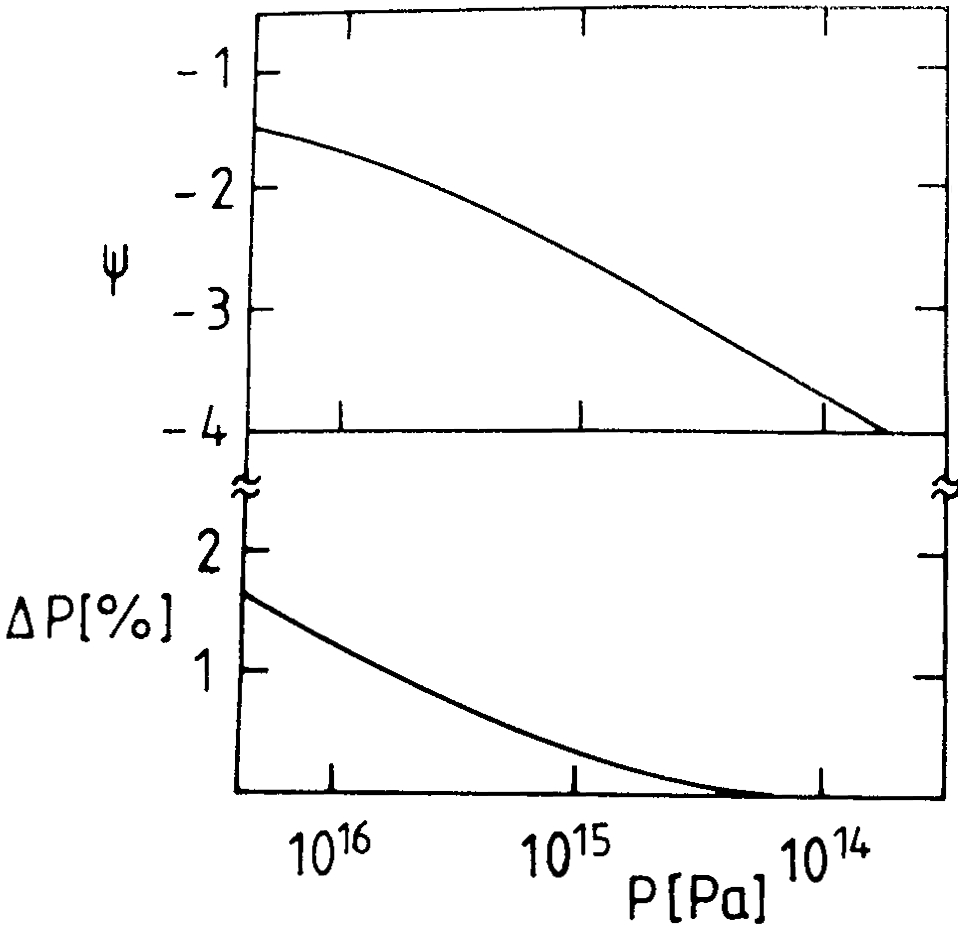
\includegraphics[width=0.5\textwidth]{degenpsiP}
        \caption{Parametro di degenerazione $\Psi$ e correzioni alla pressione dovute alla degenerazione degli elettroni nell'interno solare.}
    \end{subfigure}%
    ~
    \begin{subfigure}[t]{0.5\textwidth}
        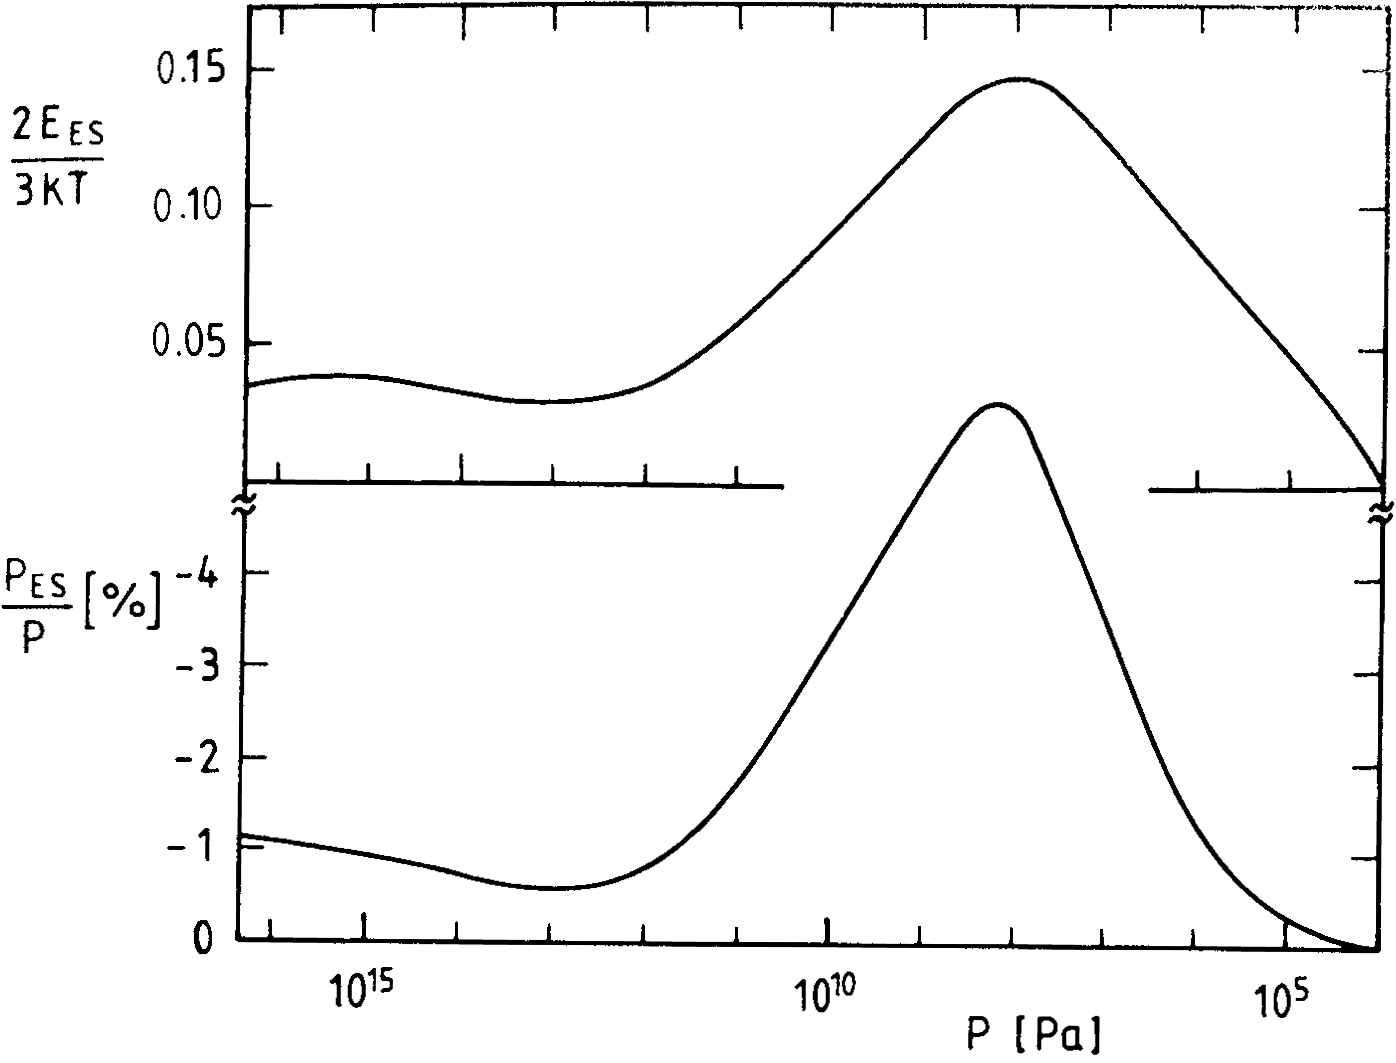
\includegraphics[width=0.6\textwidth]{RatioelectroEP}
        \caption{Rapporto fra energia termica e coulombiana la prima e fra pressione e correzione coulombiana la seconda.}
    \end{subfigure}
\end{figure*}


Il contributo degli elettroni, detta $n_e$ la densit\'a numerica, $\psi$ il parametro di degenerazione, funzinione P e T, tale che per $\psi\to-\infty$ si abbia la distribuzione di Boltzmann e per $\psi\to+\infty$ completa degenerazione, e $u_k$ energia cinetica dell'elettrone, \'e determinato da
\begin{align}
&\rho N_A\frac{1+X}{2}=\intzi{}\frac{8\pi p^2\,dp}{h^3(\exp{\frac{u_k}{KT}-\psi}+1)},\ \beta P-\rho\gasconstant{}(X+\frac{Y}{4}+\frac{Z}{\exv{A_Z}})=\frac{1}{3}\intzi{}pn_e\TDy{p}{u_k}\,dp\shortintertext{dove ho introdotto il peso atomico medio per elettrone libero (ionizzato) $\mu_e$ con}\nonumber
&\frac{1}{\mu_e}\approx X+\frac{1}{2}Y+\frac{1}{2}(1-X-Y)=\frac{1+X}{2}
\end{align}


Introduco una correzione duvuta all'interazione Coulombiana seguendo Debye-H\"uckel: il potenziale $V_i(r)$ dovuto allo ione $Z_i$ \'e schermato dagli elettroni quindi, per la formula di Boltzmann, la densit\'a degli ioni con carica Z \'e $n_Z=\overline{n}_Z\exp{-\frac{ZeV_i}{kT}}$, con $\overline{n}_Z$ densit\'a numerica dello ione $Z$ imperturbata. Assumendo l'energia coulombiana molto minore dell'energia termica espando $n_Z$ al prim'ordine nell'equazione di Poisson per $V_i$ 

\begin{align}
&\nabla^2V_i=-4\pi e\sum Zn_Z\approx\frac{1}{r_D^2}V_i\shortintertext{da cui ottengo il potenziale generato dalla nube di cariche attorno a Z}\nonumber\\
&\phi_Z=-\frac{eZ}{r_D}\shortintertext{dove}\nonumber\\
&\frac{1}{r_D^2}=\frac{4\pi e^2}{kT}\sum Z^2\overline{n}_Z=\frac{4\pi e^2}{kT}\zeta,\ \zeta=\sum_{i}(Z_i^2+Z_i)\frac{\rho X_i}{A_i}N_A
\end{align}

Le correzioni dovute alle interazioni coulombiane sono
\begin{align}
&u=\frac{3}{2}\frac{\gasconstant{}T}{\mu}+u_c,\ P=\frac{\rho}{\mu}kT+P_c\shortintertext{con}\nonumber\\[-2\normalbaselineskip]
&u_c=\frac{1}{2}\sum_ZeZ\overline{n}_Z\phi_Z=-e^3\sqrt{\frac{\pi\rho}{kT}}(N_A\zeta)\expy{\frac{3}{2}},\ P_c=\frac{1}{3}u_c
\end{align}


I fenomeni che contribuiscono all'opacit\'a nel Sole sono:

 lo scattering di fotone-elettrone che classicamente \'e descritto come lo scattering di un'onda elettromagnetica piana da parte di un dipolo oscillante, scattering Thomson,
\begin{equation}
\kappa_{\nu}\propto\frac{r_e^2}{\mu_em_u}
\end{equation}

e l'approssimazione non relativistica \'e valida per $T<\SI{e8}{\kelvin}$;

l'assorbimento di un fotone da parte di un elettrone libero \'e energeticamente possibile quando l'elettrone \'e vicino ad uno ione, l'opacit\'a in questo caso ha l'andamento

\begin{equation}
\kappa_{ff}\propto\rho T\expy{-\frac{7}{2}}
\end{equation}

si tiene conto degli effetti quantistici tramite un opportuno coefficiente, il fattore di Gaunt;

eccitazione di un elettrone o ionizzazione;

la presenza di metalli con potenziale di ionizzazione minore di H ed He rendono disponibile elettroni per la formazione di $H^-$, sistema debolmente legato per cui un fotone con $h\nu>\SI{0.75}{\ev}$ o $\lambda<\SI{1655}{\nano\meter}$ pu\'o essere assorbito: temperature di qualche $eV$ (??).

La conduzione pu\'o essere trascurata in quanto nel Sole $l_{ph}\gg l_{e}$.

\tpc{ht!}{

\node (opint) at (7,6) {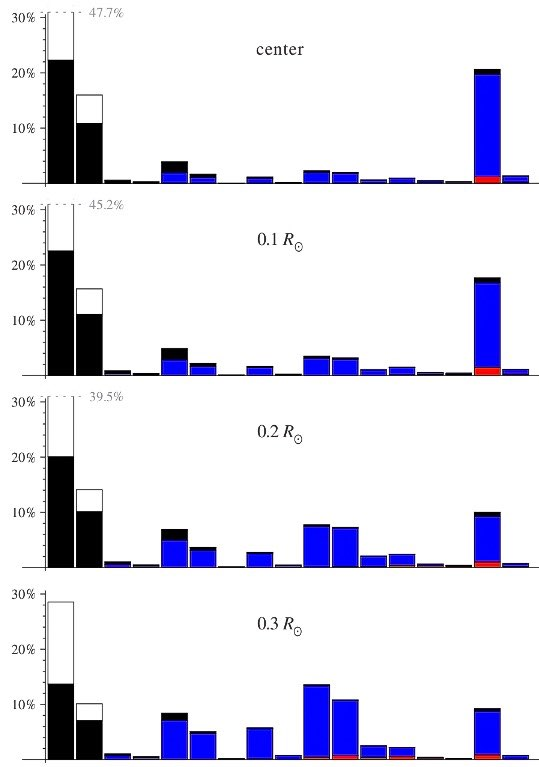
\includegraphics[width=0.5\textwidth]{opcontrib-int}};
\node at (opint.north) {(a)};
\node (opout) at (0,-6) {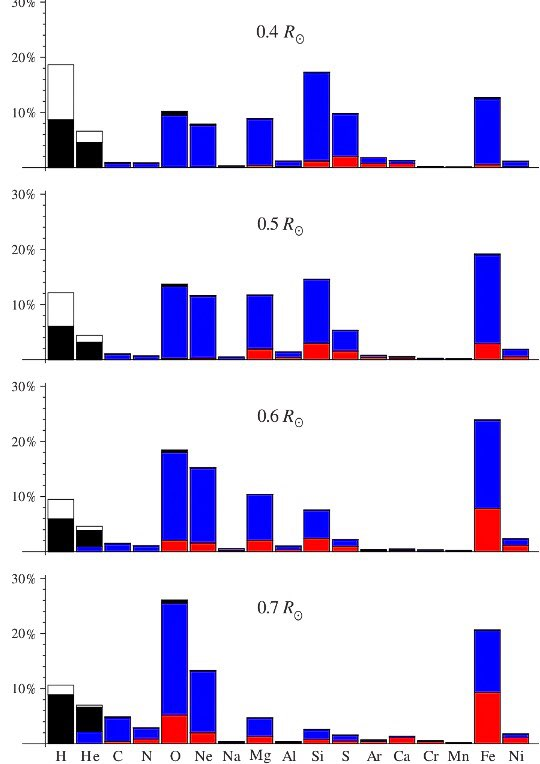
\includegraphics[width=0.5\textwidth]{opcontrib-out}};
\node[name=hydrogen, right= 8mm of opint.south west] {\tiny H};
\node[name=helium, right=4.3mm of hydrogen.west] {\tiny He};
\node[name=carbonium, right=4.3mm of helium.west] {\tiny C};
\node[name=nitrum, right=4.3mm of carbonium.west] {\tiny N};
\node[name=oxygen, right=4.3mm of nitrum.west] {\tiny O};
\node[name=neon, right=4.3mm of oxygen.west] {\tiny Ne};
\node[name=sodium, right=4.3mm of neon.west] {\tiny Na};
\node[name=magnesium, right=4.3mm of sodium.west] {\tiny Mg};
\node[name=alluminium, right=4.3mm of magnesium.west] {\tiny Al};
\node[name=silicium, right=4.3mm of alluminium.west] {\tiny Si};
\node[name=sulfur, right=4.3mm of silicium.west] {\tiny S};
\node[name=argon, right=4.3mm of sulfur.west] {\tiny Ar};
\node[name=calcium, right=4.3mm of argon.west] {\tiny Ca};
\node[name=cromum, right=4.3mm of calcium.west] {\tiny Cr};
\node[name=manganese, right=4.3mm of cromum.west] {\tiny Mn};
\node[name=ferrum, right=4.3mm of manganese.west] {\tiny Fe};
\node[name=nikel, right=4.3mm of ferrum.west] {\tiny Ni};
}{(0,-13)}{9cm}{Importanza dei varii contributi all'opacit\'a nell'interno solare.}
    
\endgroup


\section{Trasporto radiativo.}

Nell'interno stellare il cammino libero medio dei fotoni \'e molto corto $\frac{1}{\kappa\rho}\ll \rsun{}$, con l'opacit\'a $\kappa$ che descrive l'assorbimento per unit\'a di massa, quindi considero la radiazione localmente in equilibrio con la materia: il flusso di energia verso la superficie \'e generato da una piccola anisotropia nell'intensit\'a descritta al prim'ordine tramite
\begin{equation}
I_{\nu}=B(\nu,T)-\frac{1}{\kappa_{\nu}'\rho}\nabla B(\nu,T)
\end{equation}

integrando sull'angolo solido, il flusso di energia risulta

\begin{align}
&\vec{F}_{\nu}=-\frac{4\pi}{3\kappa_{\nu}\rho}\nabla B(\nu,T)\shortintertext{e integrando sulle frequenze}\nonumber\\
&\vec{F}=-[\frac{4\pi}{3\rho}\intzi{}\frac{1}{\kappa_{\nu}}\PDy{T}{B(\nu,T)}\,d\nu]\nabla T\label{eq:radiativeflux}
\end{align}

\begingroup
\color{grey}

Definisco l'opacit\'a media di Rosseland

\begin{equation}
\frac{1}{\kappa}=(\intzi{}\PDy{T}{B(\nu,T)})\expy{-1}\intzi{}\,d\nu\frac{1}{\kappa_{\nu}}\PDy{T}{B(\nu,T)}=(\frac{acT^3}{\pi})\expy{-1}\intzi{}\,d\nu\frac{1}{\kappa_{\nu}}\PDy{T}{B(\nu,T)}\label{eq:rosselandopacity}
\end{equation}

\endgroup

quindi riscrivo \eqref{eq:radiativeflux} utilizzando la pressione di radiazione $p_{rad}=\int\,d\nu\frac{4\pi}{3c}B_{\nu}=\frac{1}{3}aT^4$

\begin{align}
&\vec{F}=-\frac{4\pi}{3\kappa\rho}\nabla B=-\frac{4\pi}{3\kappa\rho}\nabla B=-\frac{c}{\kappa\rho}\nabla P_{rad}\shortintertext{che per una distribuzione sferica di materia diventa}\nonumber\\
&F_r=-\frac{c}{\kappa\rho}\TDof{r}(\frac{1}{3}aT^4)=-\frac{4acT^3}{3\kappa\rho}\TDy{r}{T}\label{eq:radfluxTgradrelation}
\end{align}

Definisco il gradiente radiativo a partire da \eqref{eq:radfluxTgradrelation}

\begin{equation}
\nrad{}=\Dcvar{\PDly{P}{T}}{rad}=\frac{3}{16\pi acG}\frac{\kappa l(r)P}{m(r)T^4}\label{eq:radiativegradient}
\end{equation}

con $l(r)=4\pi r^2F$ luminosit\'a totale in funzione di r.


\section{Condizione di in-stabilit\'a dinamica: trasporto convettivo.}

Considero sotto quali condizioni una perturbazione radiale infinitesima di un elemento di fluido cresce esponenzialmente a causa della forza di galleggiamento 
\begin{equation}
\rho\PtwoDy{t}{(\Delta r)}=-g\Delta\rho=-g[\Dcvar{\TDy{r}{\rho}}{e}-\Dcvar{\TDy{r}{\rho}}{amb}]\Delta r
\end{equation}

La forza di archimede ha direzione opposta alla perturbazione se $\Delta\rho>0$.

Considero un'equazione di stato generica $\rho(P,T,\mu)$ e definisco i coefficienti $\alpha,\delta,\phi$ tramite:
\begin{equation}
\frac{d\rho}{\rho}=\alpha\frac{dP}{P}-\delta\frac{dT}{T}+\phi\frac{d\mu}{\mu}\label{eq:deltatherm}
\end{equation}

Considero il moto dell'elemento in equilibrio di pressione con l'ambiente e, definiti i gradienti termici per il blob e l'ambiente e il gradiente di composizione chimica 

\begin{align}
&\nabla=\Dcvar{\TDly{P}{T}}{amb},\ \nabla_e=\Dcvar{\TDly{P}{T}}{blob},\ \nmu{}=\Dcvar{\TDly{P}{\mu}}{amb}\label{eq:nablavitense}\shortintertext{riscrivo l'equazione del moto}\nonumber\\
&\PtwoDy{t}{(\Delta r)}=-g\frac{\delta}{H_P}[\nabla_e-\nabla-\frac{\phi}{\delta}\nmu{}]\Delta r\label{eq:galleggiamento}
\end{align}

Suppongo adesso un moto del blob adiabatico $\nabla_e=\nabla_{ad}=\frac{P\delta}{T\rho c_P}$ e introduco la frequenza di \bv{}:
\begin{align}
&N^2=g(\frac{1}{\Gamma_1P}\TDy{r}{P}-\frac{1}{\rho}\TDy{r}{\rho})\label{eq:bvfs}\\
&N^2=g(\frac{1}{\densityscale{}}-\frac{g}{c_s^2})\label{eq:bvfsdensita}\shortintertext{ho definito le lunghezze caratteristiche per variazione di densit\'a e pressione:}\nonumber\\
&\densityscale{}=-\frac{dr}{d\ln{\rho}},\ H_P=-\frac{dr}{dP}
\end{align}

$N^2$ rappresenta la massima frequenza sotto cui pu\'o oscillare una particella di fluido sottoposta a onde di gravit\'a mantenendo l'equilibrio di pressione con l'ambiente.

La variazione di composizione ambientale pu\'o essere descritta tramite $\densityscale{}$ in \eqref{eq:bvfsdensita}, quindi riscrivo l'equazione \eqref{eq:galleggiamento}
\begin{equation}
\PtwoDy{t}{(\Delta r)}=-N^2\Delta r
\end{equation}
che descrive un comportamento oscillatorio per $N^2>0$, cio\'e uno strato di gas del Sole \'e stabile per convezione se

\begin{equation}
\nrad{}<\nad+\frac{\phi}{\delta}\nmu{}\label{eq:ledoux}
\end{equation}

dove ho usato $\nabla_{amb}=\nrad{}$ definito in \eqref{eq:radiativegradient}, cio\'e il gradiente che si ha nel caso la luminosit\'a si trasportata dai fotoni.

\begin{figure}[!h]
\begin{subfigure}[t]{0.5\linewidth}
\centering
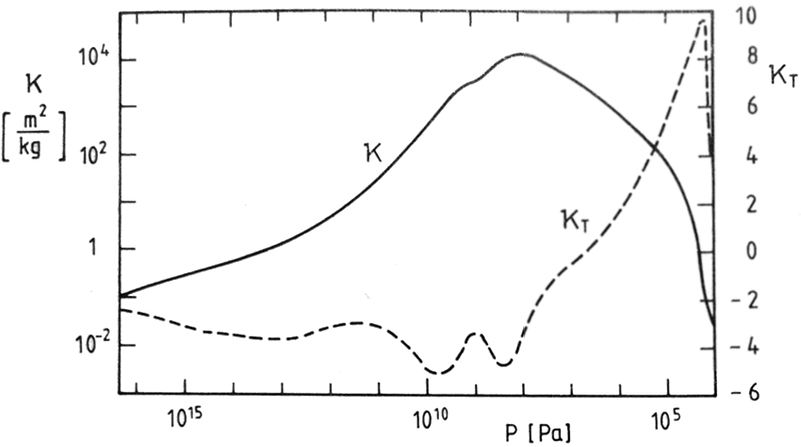
\includegraphics[keepaspectratio,width=0.9\linewidth]{opacitylld}
\subcaption{Profilo radiale di $\kappa$ e $\PDly{T}{\kappa}$. Da \cite{sti91sun}.}
\end{subfigure}
~
\begin{subfigure}[t]{0.5\linewidth}
\centering
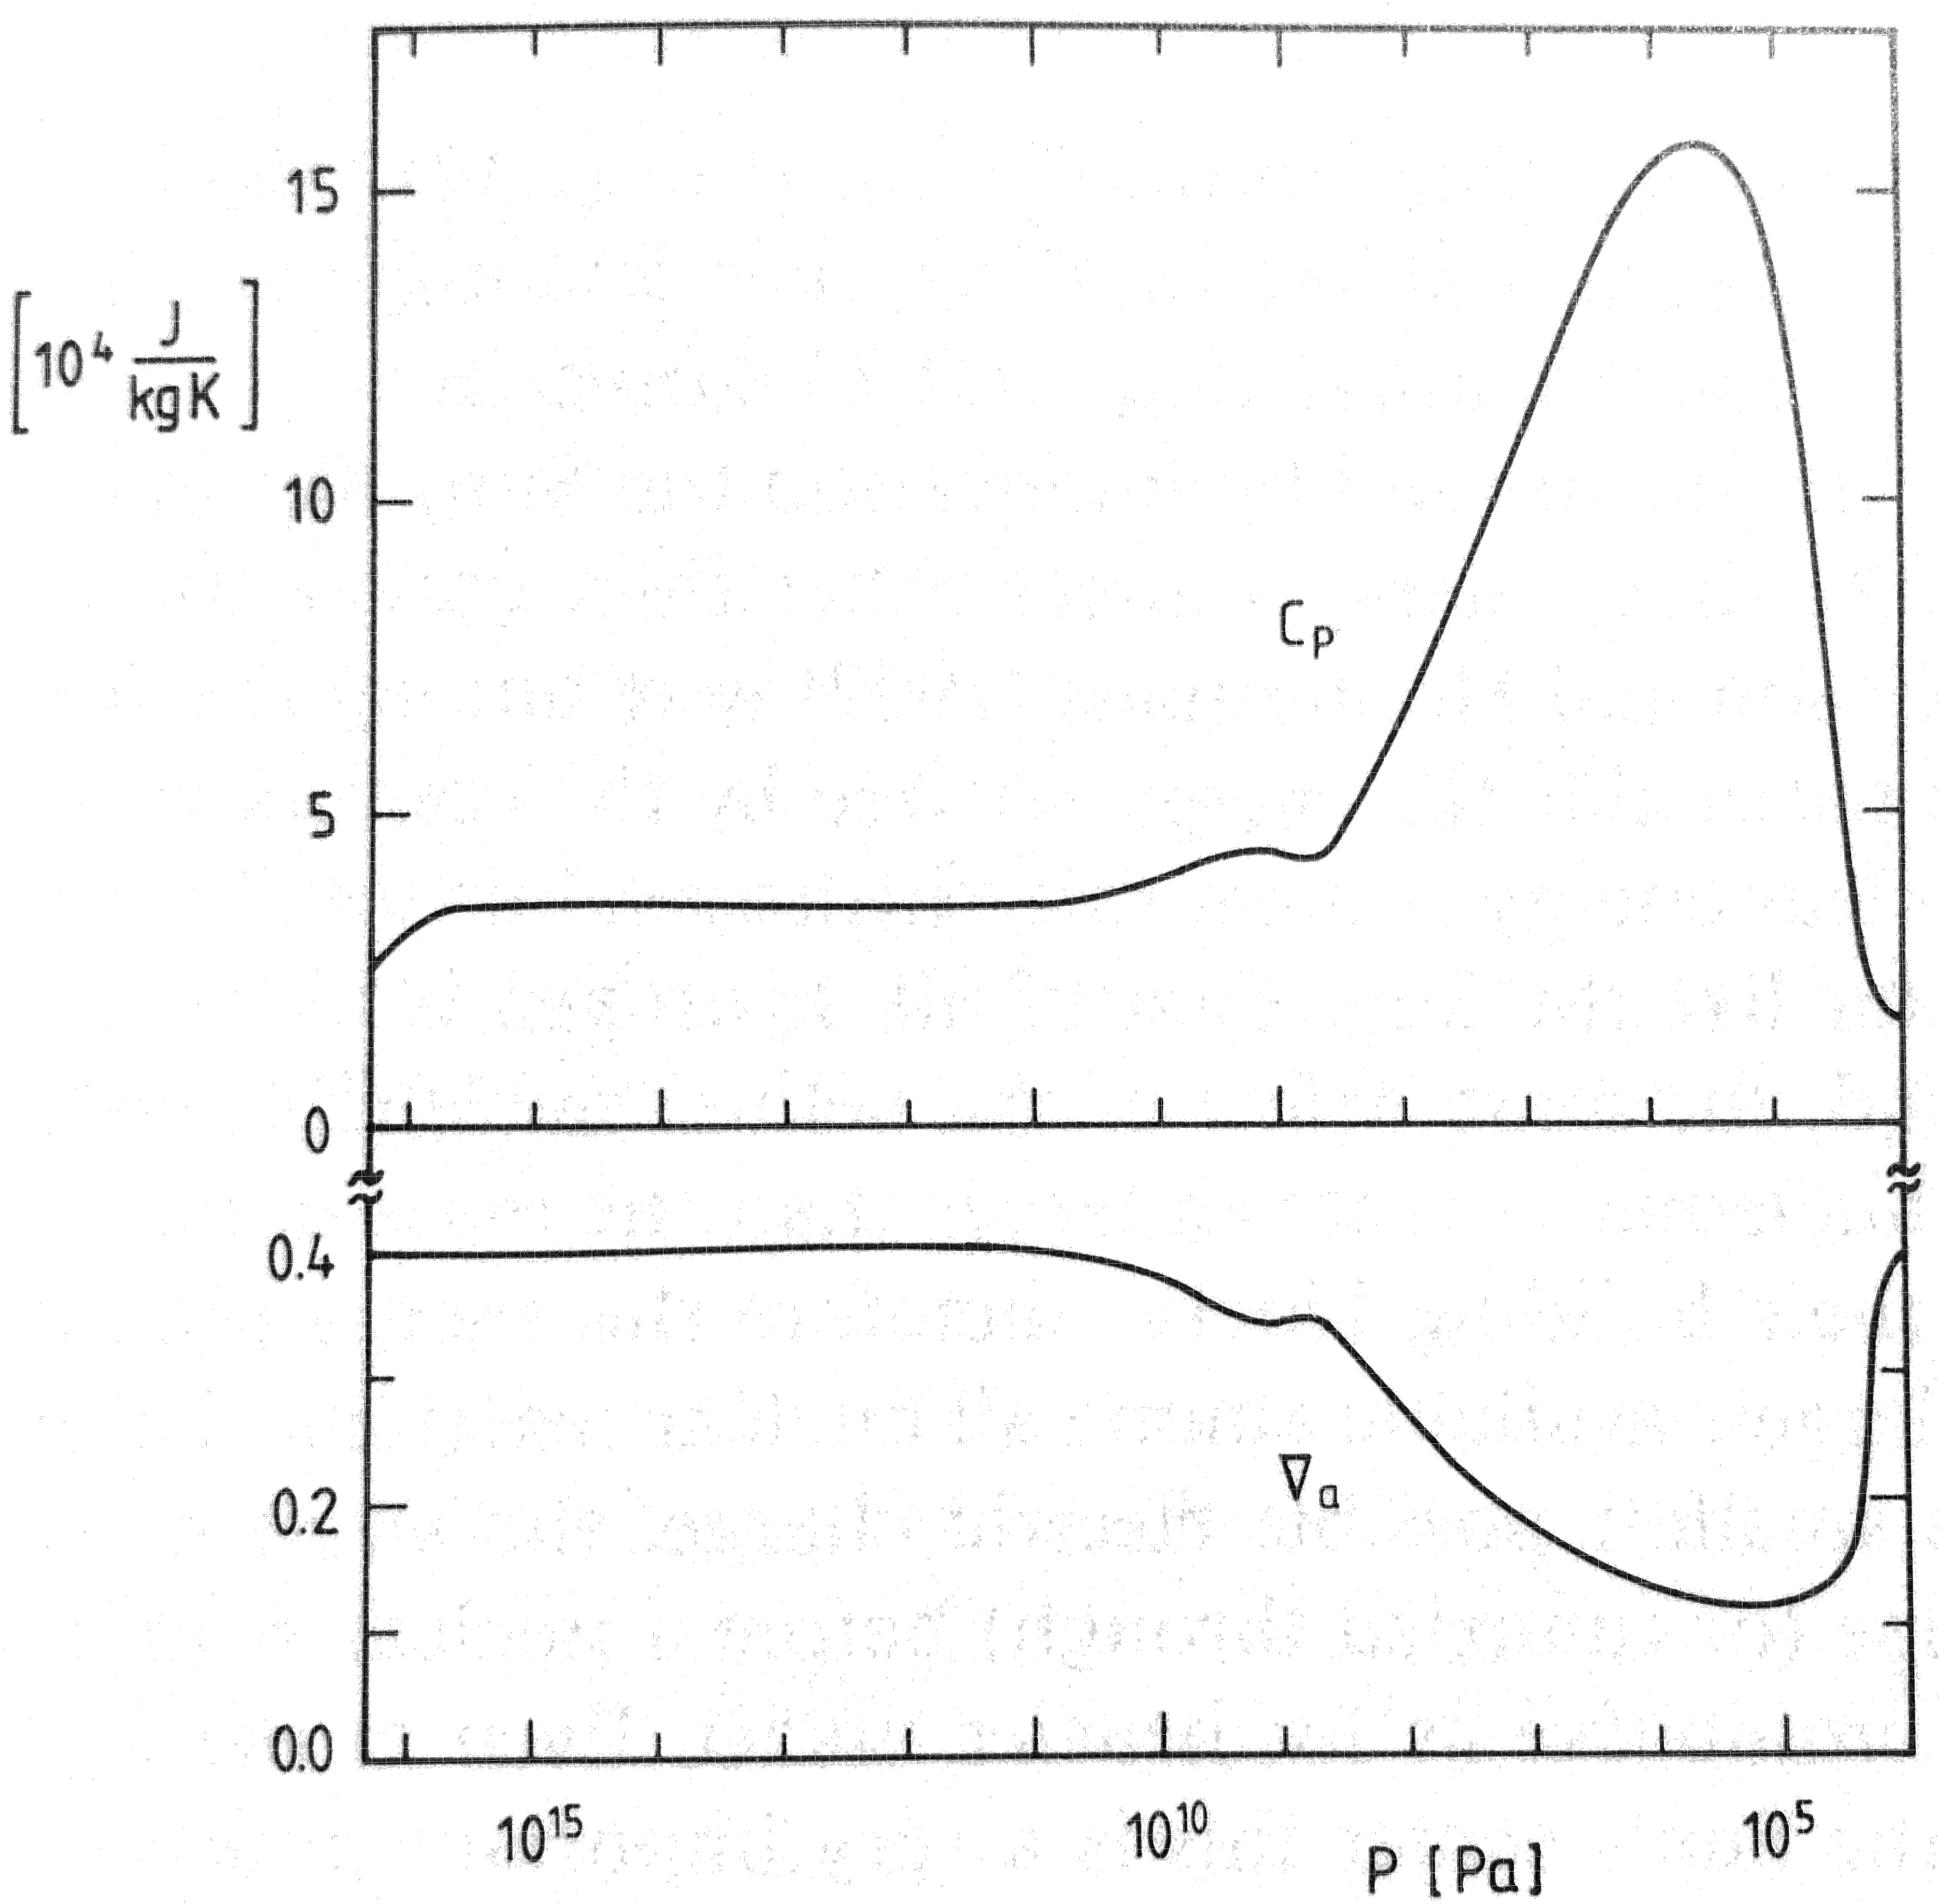
\includegraphics[keepaspectratio,width=0.7\linewidth]{specificheatnablaa}
\subcaption{Profilo radiale di $c_P$ e $\nabla_a$. Da \cite{sti91sun}.}
\end{subfigure}
    
\end{figure}

\subsection{Teoria della mixing-length}

La zona convettiva occupa il $29\%$ pi\'u esterno del raggio solare e il $2\%$ della massa: questa regione \'e chimicamente omogenea a causa dei moti convettivi. Le basse temperature causano un aumento dell'opacit\'a e il gradiente termico necessario per trasportare la luminosit\'a solare \'e superiore al gradiente adiabatico, il cui valore \'e diminuito dal calore latente dell'idrogeno solo parzialmente ionizzato.

Una maggiore efficienza del trasporto convettivo di energia si riflette in una minore differenza tra il gradiente di temperature adiabatico ed effettivo: per determinare lo scostamento dalla stratificazione adiabatica dovuto alle perdite radiative utilizzo la teoria della mixing-length.

Il flusso di energia complessivo \'e determinato da
\begin{equation}
F_{con}+F_{rad}=\frac{4acG}{3}\frac{T^4m}{\kappa Pr^2}\nrad{}\label{eq:totalflux}
\end{equation}

Per determinare il gradiente di temperatura effettivo $\nabla$ uso la teoria della mixing-length (\cite{prandtl25tur} e \cite{vitense53kon}):
si considera l'eccesso di calore trasportato dai blob di gas nel moto convettivo $c_P\Delta T$ rispetto all'ambiente, il cui cammino libero medio \'e la mixing-length $l_m=\alpha H_P$, che da luogo al flusso di energia
\begin{equation}
F_{con}=\exv{\rho vc_P\Delta T}\label{eq:convectiveflux}
\end{equation}
dove $\exv{}$ indica una media opportuna sul guscio sferico di raggio r. Determino il valor medio della differenza di temperatura prendendo come valore caratteristico dello spostamento del blob di gas $\Delta r\approx\frac{l_m}{2}$:
\begin{equation}
\frac{\Delta T}{T}\approx\frac{1}{T}\PDy{r}{(\Delta T)}\frac{l_m}{2}=(\nabla-\nabla_e)\frac{l_m}{2}\frac{1}{H_P}
\end{equation}

Assumo il lavoro medio fatto dalla forza di galleggiamento per unit\'a di massa $-g\frac{\Delta\rho}{\rho}$ uguale al valore medio della forza, cio\'e la met\'a di quello al guscio sferico dato, moltiplicato lo spostamento medio $\frac{l_m}{2}$ quindi, assumendo in oltre che in media met\'a del lavoro fatto dalla forza di galleggiamento sia trasformato in energia cinetica del blob si ottiene
\begin{equation}
v^2=g\delta(\nabla-\nabla_e)\frac{l_m^2}{8H_P}\label{eq:blobvelocity}
\end{equation}

Infine determino gli scambi radiative del blob: il modulo del flusso radiativo \'e proporzionale al gradiente termico in direzione normale alla superficie del blob
\begin{equation}
f=\frac{4acT^3}{3\kappa\rho}|\PDy{n}{T}|
\end{equation}

quindi l'energia scambiata dall'intera superficie S del blob \'e $\lambda=Sf$ che determina, per la prima legge della termodinamica, una variazione di temperatura per unit\'a di tempo, indicato con $V$ il volume, $\PDy{t}{T_e}=-\frac{\lambda}{\rho Vc_P}$.

La variazione della temperatura del blob per unit\'a distanza percorsa \'e quindi
\begin{equation}
\Dcvar{\TDy{r}{T}}{e}=\Dcvar{\TDy{r}{T}}{ad}-\frac{\lambda}{\rho Vc_Pv}\label{eq:Tchangelength}
\end{equation}
esplicitando $\lambda$ approssimando il gradiente normale alla superficie con $\exv{\Delta T}$ ed usando le definizioni \eqref{eq:nablavitense} si ottiene
\begin{equation}
\frac{\nabla_e-\nad{}}{\nabla-\nabla_e}=\frac{6acT^3}{\kappa\rho^2c_Pl_mv}
\end{equation}

Le 5 equazioni \eqref{eq:totalflux},\eqref{eq:radiativegradient}, \eqref{eq:convectiveflux}, \eqref{eq:blobvelocity}, \eqref{eq:nablavitense} determinano completamente le variabili $F_{rad}, F_{con}, v, \nabla_e, \nabla$ in funzione di $P,T,l(r),m(r),c_P,\nad{},\nrad{},g$ .

\begin{minipage}{\linewidth}
\makebox[\linewidth]{
    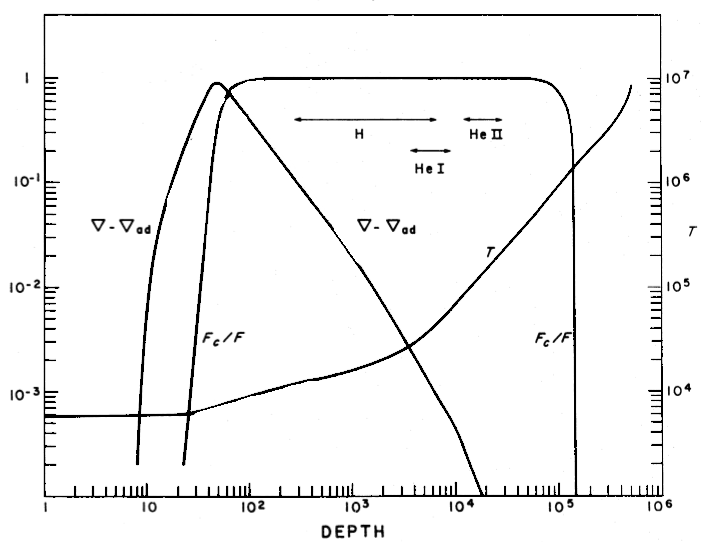
\includegraphics[height=0.4\textheight,keepaspectratio]{proportionflux}}
    \captionof{figure}{Da \cite{gou76convection}}
    \label{fluxproportion}
\end{minipage}

\begingroup
\color{grey}
section(Descrizione dello stato del gas solare)
\endgroup

\section{Calibrazione del modello solare e incertezze}

\begingroup
\color{grey}
\subsection{Equazione di stato}

Per determinare l'equazione di stato esistono due approcci: lo schema chimico considera atomi e molecole, ricava l'energia libera del sistema, e minimizzando l'energia libera si ottengono relazioni termodinamiche ed equazione di stato, utilizzando questo approccio \'e stata ricavata l'equazione di stato MHD; lo schema fisico considera nuclei ed elettroni come costituenti fondamentali interagenti tramite potenziale Coulombiano e trova le soluzione dell'equazione di Schr\"oedinger per un problema a molti corpi, questo approccio, usato per ricavare l'equazione di stato OPAL, \'e pi\'u adatto per trattare le regioni interne del Sole.

''descrivo sommariamente i varii contributi''

In questa tesi scrivo un'espressione approssimata tenendo conto delle correzioni all'equazione di stato dei gas perfetti per l'interazione Coulombiana e la degenerazione degli elettroni, illustro i processi che causano l'evoluzione chimica, e determinano il tempo di vita in sequenza principale del Sole mentre non considero i i meccanismi responsabili dell'opacit\'a e gli effetti della pressione di radiazione sulla diffusione degli ioni.

Considero il contributo alla pressione degli ioni, degli elettroni degeneri nella parte interna del Sole, e dei fotoni, $P=P_I+P_R+P_e$, dove ho
\begin{align}
&P_I=\rho \gasconstant{} T(X+\frac{Y}{4}+\frac{Z}{\exv{A_Z}})\shortintertext{dove ho usato il peso molecolare medio per i soli ioni $\mu_0$,}\nonumber\\
&P_R=\frac{a}{3}T^4\shortintertext{definisco il parametro $\beta$}\nonumber\\
&P_R=(1-\beta)P
\end{align}

Il peso molecolare medio, definito come massa media in amu per particella libera \'e

\begin{align}
&\mu=\frac{1}{\bar{n}_HX+\bar{n}_{He}Y+\bar{n}_{Z}Z}\label{eq:meanmw}\intmy{con $\bar{n}_i=\frac{1+f_i}{A_i}$ numero medio di particelle libere per unit\'a di massa atomica dovute alla specie i di peso atomico $A_i$ con $f_i$ numero medio di elettroni liberati da specie i.}\nonumber
\end{align}

    \begin{figure*}[!h]
    \centering
  \begin{subfigure}[t]{0.5\textwidth}
        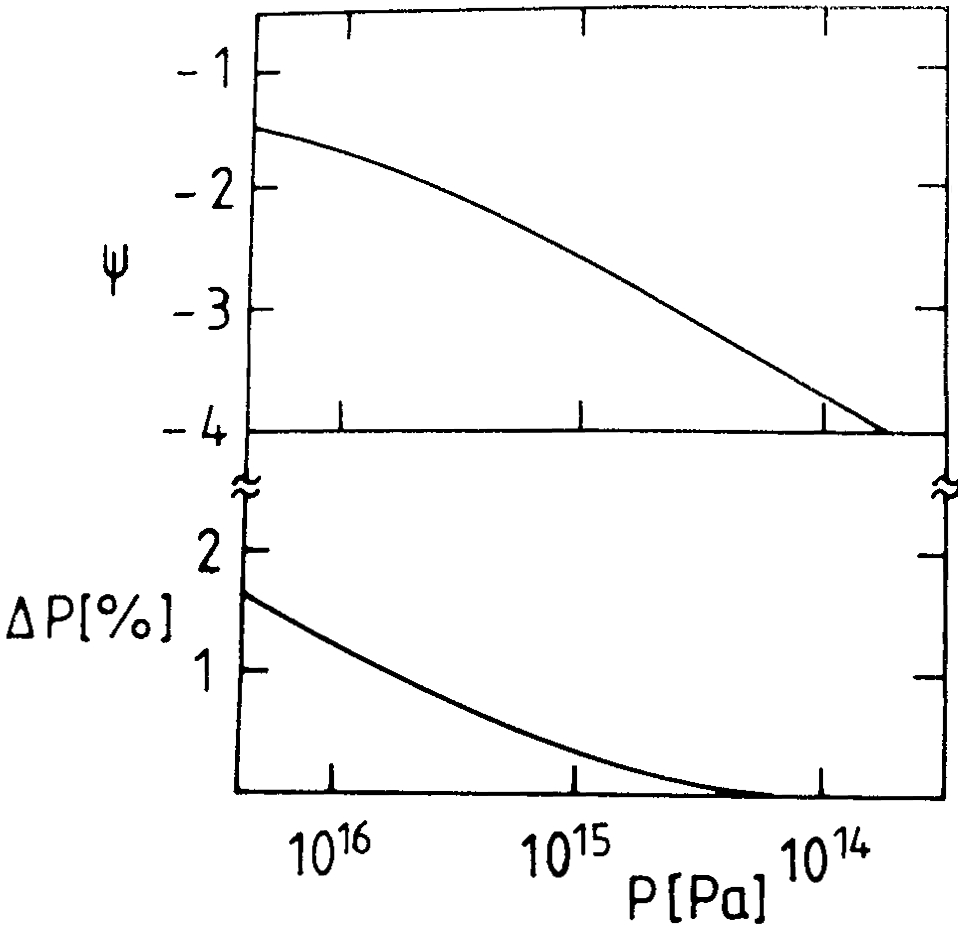
\includegraphics[width=0.5\textwidth]{degenpsiP}
        \caption{Parametro di degenerazione $\Psi$ e correzioni alla pressione dovute alla degenerazione degli elettroni nell'interno solare.}
    \end{subfigure}%
    ~
    \begin{subfigure}[t]{0.5\textwidth}
        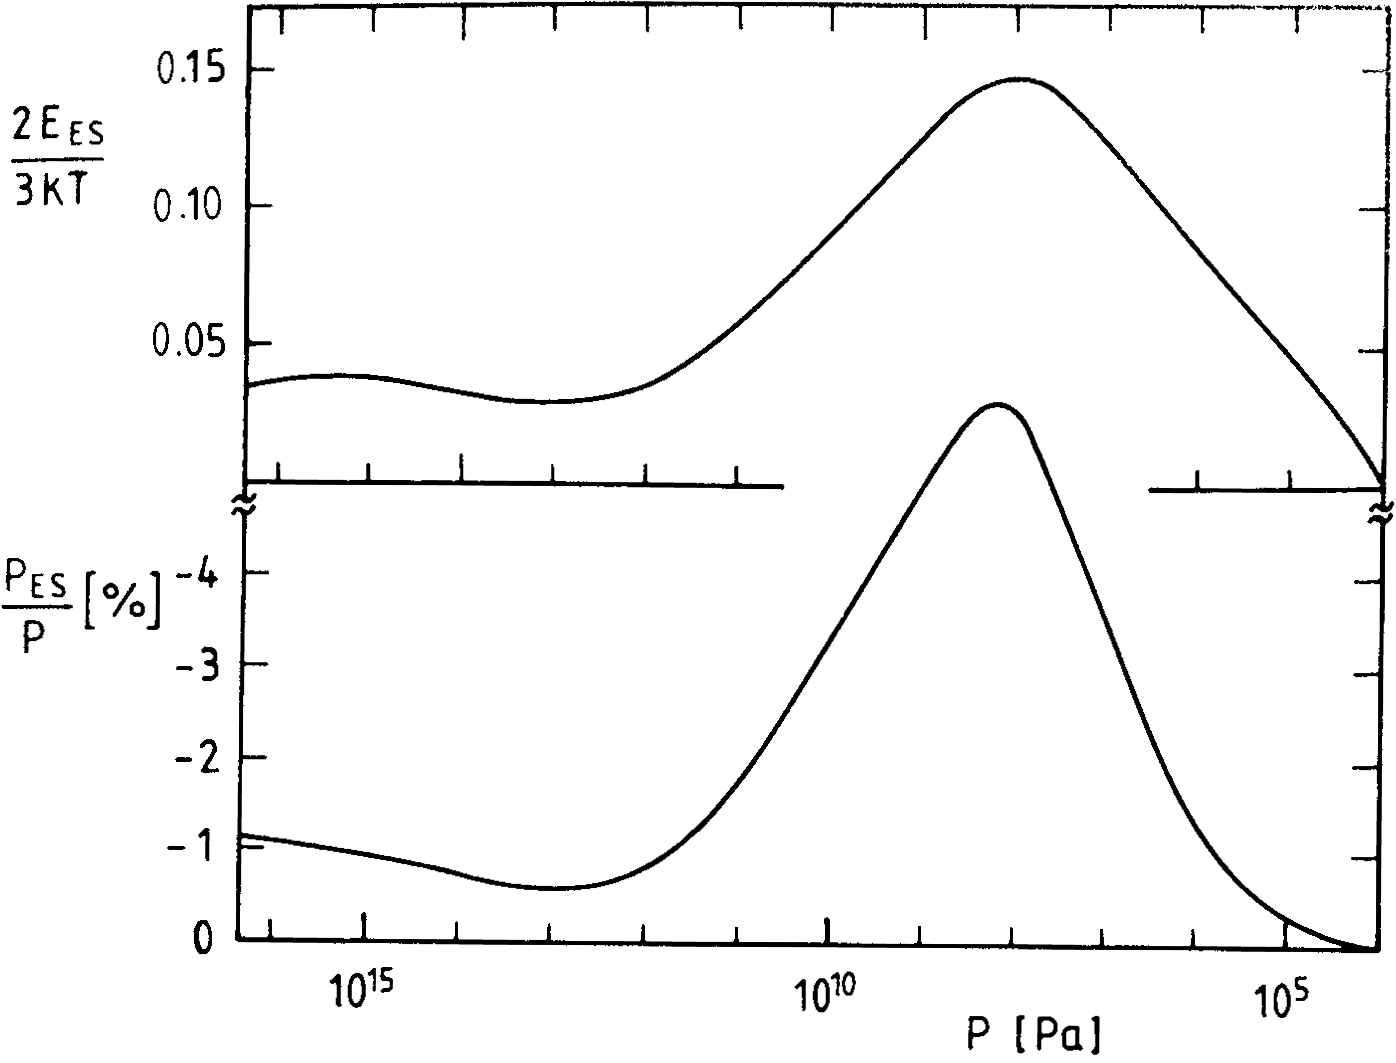
\includegraphics[width=0.6\textwidth]{RatioelectroEP}
        \caption{Rapporto fra energia termica e coulombiana la prima e fra pressione e correzione coulombiana la seconda.}
    \end{subfigure}
\end{figure*}


Il contributo degli elettroni, detta $n_e$ la densit\'a numerica, $\psi$ il parametro di degenerazione, funzinione P e T, tale che per $\psi\to-\infty$ si abbia la distribuzione di Boltzmann e per $\psi\to+\infty$ completa degenerazione, e $u_k$ energia cinetica dell'elettrone, \'e determinato da
\begin{align}
&\rho N_A\frac{1+X}{2}=\intzi{}\frac{8\pi p^2\,dp}{h^3(\exp{\frac{u_k}{KT}-\psi}+1)},\ \beta P-\rho\gasconstant{}(X+\frac{Y}{4}+\frac{Z}{\exv{A_Z}})=\frac{1}{3}\intzi{}pn_e\TDy{p}{u_k}\,dp\shortintertext{dove ho introdotto il peso atomico medio per elettrone libero (ionizzato) $\mu_e$ con}\nonumber
&\frac{1}{\mu_e}\approx X+\frac{1}{2}Y+\frac{1}{2}(1-X-Y)=\frac{1+X}{2}
\end{align}


Introduco una correzione duvuta all'interazione Coulombiana seguendo Debye-H\"uckel: il potenziale $V_i(r)$ dovuto allo ione $Z_i$ \'e schermato dagli elettroni quindi, per la formula di Boltzmann, la densit\'a degli ioni con carica Z \'e $n_Z=\overline{n}_Z\exp{-\frac{ZeV_i}{kT}}$, con $\overline{n}_Z$ densit\'a numerica dello ione $Z$ imperturbata. Assumendo l'energia coulombiana molto minore dell'energia termica espando $n_Z$ al prim'ordine nell'equazione di Poisson per $V_i$ 

\begin{align}
&\nabla^2V_i=-4\pi e\sum Zn_Z\approx\frac{1}{r_D^2}V_i\shortintertext{da cui ottengo il potenziale generato dalla nube di cariche attorno a Z}\nonumber\\
&\phi_Z=-\frac{eZ}{r_D}\shortintertext{dove}\nonumber\\
&\frac{1}{r_D^2}=\frac{4\pi e^2}{kT}\sum Z^2\overline{n}_Z=\frac{4\pi e^2}{kT}\zeta,\ \zeta=\sum_{i}(Z_i^2+Z_i)\frac{\rho X_i}{A_i}N_A
\end{align}

Le correzioni dovute alle interazioni coulombiane sono
\begin{align}
&u=\frac{3}{2}\frac{\gasconstant{}T}{\mu}+u_c,\ P=\frac{\rho}{\mu}kT+P_c\shortintertext{con}\nonumber\\[-2\normalbaselineskip]
&u_c=\frac{1}{2}\sum_ZeZ\overline{n}_Z\phi_Z=-e^3\sqrt{\frac{\pi\rho}{kT}}(N_A\zeta)\expy{\frac{3}{2}},\ P_c=\frac{1}{3}u_c
\end{align}

\endgroup

\begingroup
\color{midnightblue}
\subsection{Reazioni nucleari.}
\endgroup


La composizione chimica \'e modificata dalle reazioni di fusione che per gli elementi principali, assumendo condizione di equilibrio secolare, riassumo
%%% \tag{\theequation a,b}
\begin{subequations}\label{subeqn:fusionchange}
\begin{align}
&\dot{X}=\frac{m_p}{N_A}(-3r_{pp}+2r_{33}-r_{34}-4r_{p14})\\ 
&\dot{Y}_3=\frac{m_{He3}}{N_A}(r_{pp}-2r_{33}-r_{34})\\
&\dot{Y}=\frac{m_{He4}}{N_A}(r_{33}+r_{34}+r_{p14})
\end{align}
\end{subequations}

con $r_{ik}$ rate di reazione per unit\'a di massa:

\begin{align}
&r_{ik}=\frac{\rho N_A^2X_iX_k}{(1+\delta_{ik})A_iA_k}\lambda_{ik}\shortintertext{dove, introducendo il fattore astrofisico $S(E)$, la massa ridotta dei due reagenti $m_{ik}$}\nonumber\\
&\lambda_{ik}=\sqrt{\frac{8}{m_{ik}\pi}}\frac{S_{ik}|_{E=0}}{(kT)\expy{\frac{3}{2}}}\intzi{}\exp{(-\frac{E}{kT}-\frac{b}{\sqrt{E}})}\,dE,\ b=31.28Z_1Z_2\sqrt{\frac{m_{ik}}{m_u}}\,(KeV)\expy{-1}\label{eq:astrofactor}
\end{align}

\begingroup
\color{midnightblue}
incertezza su $S_{11}$
\endgroup


\subsection{Processi di diffusione.}


Oltre alle reazioni di fusioni anche i processi di diffusione modificano l'abbondanza degli elementi, il peso molecolare medio e l'opacit\'a. Sebbene il tempo caratteristico per percorre un raggio solare sia lungo $\tau_{diff}\approx\SI{6e13}{\year}$ i processi di diffusione producono effetti misurabili sulle frequenze dei modi di oscillazione: la loro inclusione nei \mss{} produce un miglior accordo con le osservazioni.

I processi di diffusione inglobano diversi effetti: la gravit\'a tende a concentrare gli elementi pi\'u pesanti verso il centro, le interazioni elettromagnetiche mantengono gli elettroni ancorati ai nuclei, la diffusione termica concentra le particelle pi\'u cariche e pi\'u pesanti nelle zone pi\'u calde, mentre la presenza di gradiente di concentrazione $C_s=\frac{n_s}{n_e}$ produce diffusione in senso opposto. Si tiene conto del flusso di massa, momento ed energia nelle equazioni di conservazione attraverso le equazioni sviluppate da Burgers (1969), per la concentrazione numerica della specie s ho un l'equazione di continuit\'a.

\begin{equation}
\PDy{t}{n_s}+\frac{1}{r^2}\PDof{r}(r^2n_sw_s)=\Dcvar{\PDy{t}{n_s}}{Nucl}\label{eq:difffusionchange}
\end{equation}

con $w_s$ velocit\'a di diffusione specie s.

\begin{minipage}{\linewidth}
\begin{tikzpicture}
\node[inner sep=0pt] (image) at (0,0)
  {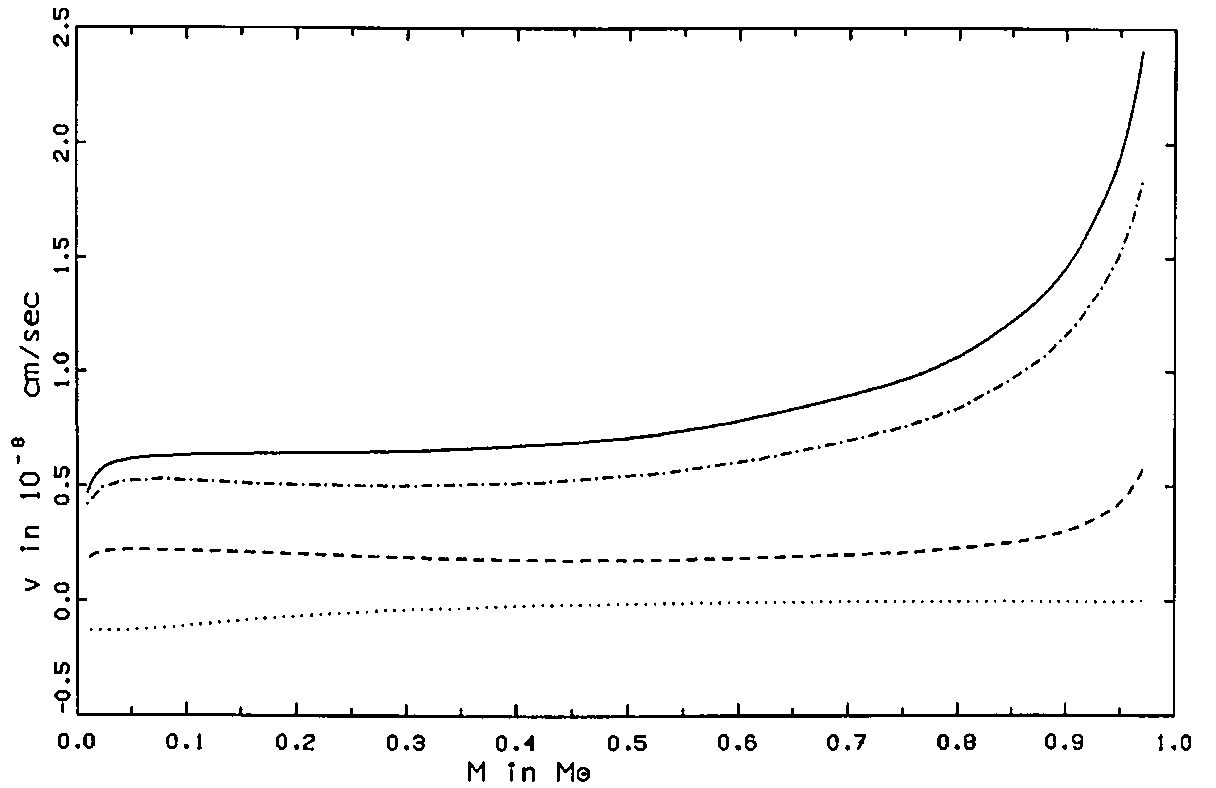
\includegraphics[keepaspectratio=true,scale=0.2]{Hdiffusion}};
  \draw [thick,dotted] (-3.4,1.5) -- (-3,1.5) node[right] {$\propto\nabla c$};
 \draw [thick,dashed] (-3.4,1.9) -- (-3,1.9) node[right] {$\propto\nabla T$};
    \draw [thick,dash dot] (-3.4,2.3) -- (-3,2.3) node[right] {$\propto\nabla P$};
    \node (caption) at (7,2) { \begin{minipage}[c]{0.3\textwidth}
\captionof{figure}{Contributi alla velocit\'a di diffusione di H-He in modello di $1\msun{}$ a \SI{4.65e9}{\year}. Da \cite{wam88hydrogen}.}%   
    \end{minipage}};
\end{tikzpicture}
\end{minipage}


\begingroup
\color{midnightblue}
stime diffusione
diffusione termica
\endgroup


\subsection{Modello solare standard.}

\begingroup
\color{grey}
simmetria sferica.

\begin{itemize*}
\item pressione gas
\item pressione turbolenta == kinetic pressure
\item radiation pressure $-->$ photon absorption
\item magnetic pressure
\end{itemize*}

\endgroup

\begingroup
\color{midnightblue}
grafico densita vs pressione bahcall95
tabella input del mss: eta, luminosita, raggio,
\endgroup

Un modello del Sole attuale si ottiene integrando numericamente le equazioni fondamentali della struttura stellare \eqref{subeqn:stellarstructure} per ottenere il profilo radiale delle grandezze $\{P,m,T,L,X_i\}$, note  l'equazione di stato $P(\rho,T,X_i)$ (e l'energia interna $u(P,T,X_i)$), l'opacit\'a $\kappa$, il rate di produzione di energia nucleare $\epsilon(P,T,X_i)$.

Descrivo le caratteristiche del trasporto di energia verso la superficie attraverso la relazione

\begin{subequations}\label{subeqn:stellarstructure}
\begin{align}
&\TDy{r}{m}=4\pi r^2\rho\\
&\TDy{r}{P}=-\frac{Gm(r)\rho(r)}{r^2}\\
&\TDy{r}{T}=\nabla\frac{T}{p}\TDy{r}{p}\\
&\TDy{r}{L}=4\pi r^2[\rho(\epsilon-\epsilon_{\nu})-\rho\TDof{t}u+\frac{P}{\rho}\TDy{t}{\rho}]
\end{align}
\end{subequations}

I meccanismi di trasporto di energia determinano il gradiente di temperatura $\nabla=\TDly{P}{T}$ fissata la luminosit\'a alla superficie.

Le condizioni al bordo sono
\begin{itemize}
    \item La superficie \'e definita da $T=T_{eff}$ e si ha la condizione $L=4\pi r^2\sigma T^4$. La pressione alla superficie \'e legata alla struttura di equilibrio dell'atmosfera.
    \item In $r=0$ deve essere $L=0$, $M=0$.
    %e condizioni al centro si ricavano espandendo l, m attorno a $r=0$ in termini di $T_c, P_C,X_C,X_{3C}$ ed eguagliando le espansioni ai valori di l e m del punto pi\'u interno.
\end{itemize}
per $X_i(r)$ e M fissati, e costruendo una sequenza evolutiva del Sole in sequenza principale fino ad ottenere un modello solare con le caratteristiche del Sole attuale:

l'aumento del peso molecolare medio $\mu$, determinato tramite \eqref{eq:difffusionchange}, dovuto principalmente alle reazioni di fusione \eqref{subeqn:fusionchange}, deve essere compensato da un'aumento di temperatura con conseguente incremento dell'energia generata e della luminosit\'a.

L'incertezza sull'abbondanza iniziale di He e sui meccanismi del trasporto convettivo rendono necessaria una calibrazione in funzione della luminosit\'a e raggio attuali. 

L'et\'a del sistema solare \'e nota grazie modelli di formazione e analisi dei meteoriti che determinano $t_{\odot}=\SI{4.9+-0.1e9}{\year}$ con incertezza dovuta al periodo di solidificazione dei meteoriti.
La luminosit\'a dipende fortemente dal valore di $Y_0$,  mentre il raggio da $\alpha$, parametro che regola l'efficienza del trasporto convettivo nella regione esterna caratterizzata fisicamente dall'entropia il cui valore \'e determinato, a meno di una costante additiva, dalla zona superadiabatica vicino alla superficie. 

Scelgo $Y_0$ e $\alpha$ che forniscono luminosit\'a e raggio $\rsun{}=\SI{6.96e8}{\meter}$ attuali del Sole: risulta $\frac{R_b}{\rsun{}}\approx0.710$ e il valore di $Y_0=0.250$.

\begingroup
\color{yellow}

\eqref{eq:massaguscio},\eqref{eq:fidroequilibrio},\eqref{eq:fenergyconservation}, \eqref{eq:ftransportenergy} a partire da $r=0$ produce soluzioni dipendenti da $(P_c,T_c)$, mentre le condizioni alla superficie sono pi\'u complesse perch\'e dipendono dalla struttura dell'atmosfera e le soluzioni sono dipendenti da $(R,L)$: i quattro parametri matematici del problema, $(P_c,T_C,L,R)$, sono determinati dalla condizione di continuit\'a ad un punto intermedio  delle soluzioni $(P,T,m(r),l(r))$ fra le soluzioni con condizioni al centro e sulla superficie.
\endgroup


\begingroup
\color{midnightblue}
Incertezze negli input del SSM e quindi su $\alpha$ e $Y$
\endgroup


\end{document}